阿托伐醌,亦作阿托喹酮或美普龙,是一种可用于治疗肺囊虫病以及疟疾、瘴气的药物。酮酯\textbf{1}和醛\textbf{2}是合成阿托伐醌的关键化合物。

\begin{figure}[h]
	\centering
	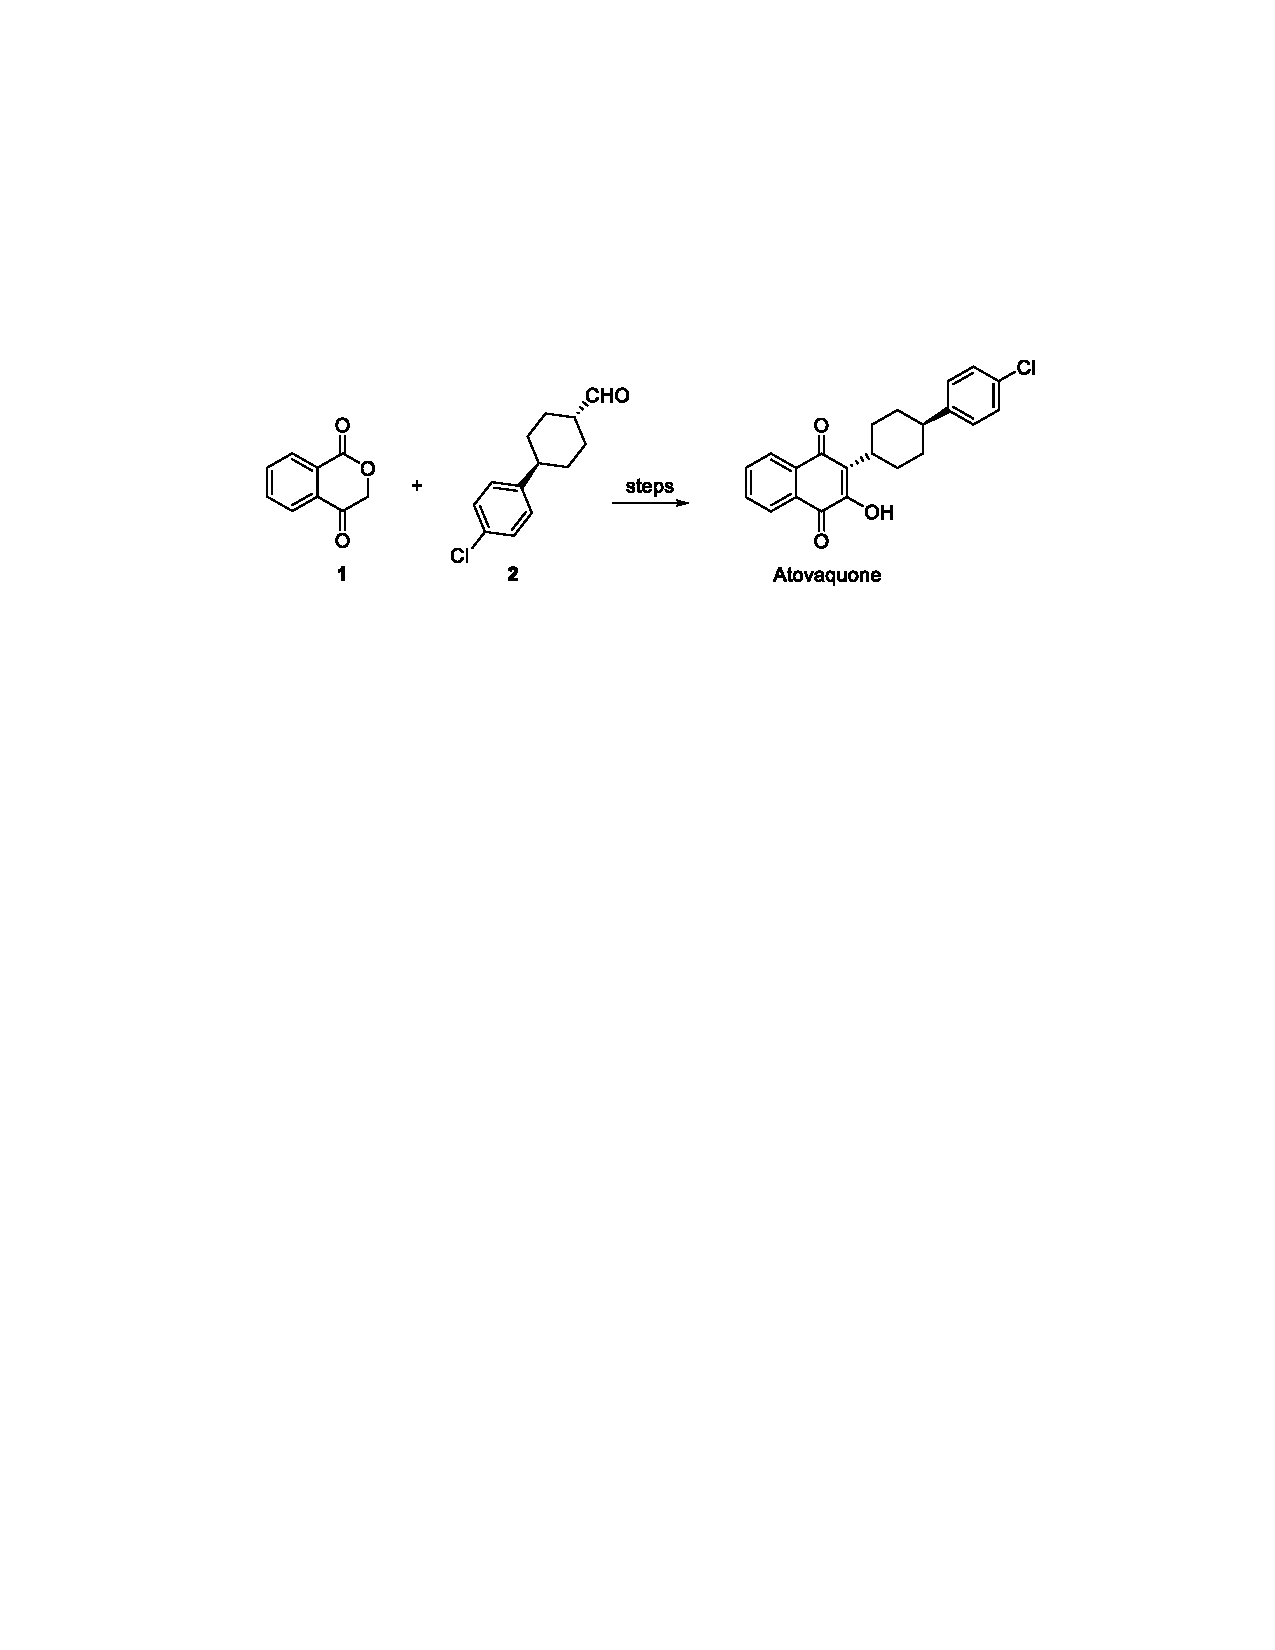
\includegraphics[width=14cm]{./pic/t6-1.pdf}
\end{figure}

关键化合物酮酯\textbf{1}的合成如下所示。将丙二酸在加热条件下加入邻苯二甲酸酐和三乙胺的混合物,在此过程中可观察到有气体逸出。以盐酸处理反应体系可经过有两个羧基的中间体\textbf{A}得到酸\textbf{3}。酸\textbf{3}可转化为分子式相同且包含半缩酮基团和酯基的中间体\textbf{B},随后脱水生成烯烃\textbf{C},再在酸性条件下溴化而生成\textbf{D}。二溴代物\textbf{D}在热的H\textsubscript{2}O/AcOH混合体系体系中溶剂解生成叔碳正离子中间体\textbf{E},随后\textbf{E}被水捕获生成中间体半缩酮\textbf{F},最后,中间体半缩酮\textbf{F}重排生成关键化合物\textbf{1}。

\noindent 注:方括号表示产物未进行分离和纯化而直接进行进一步反应。由\textbf{3}到\textbf{1}的转化是一个一锅煮反应,即不经对中间体的分离纯化而在同一个容器中一个接着一个发生的一系列反应。

\begin{figure}[h]
	\centering
	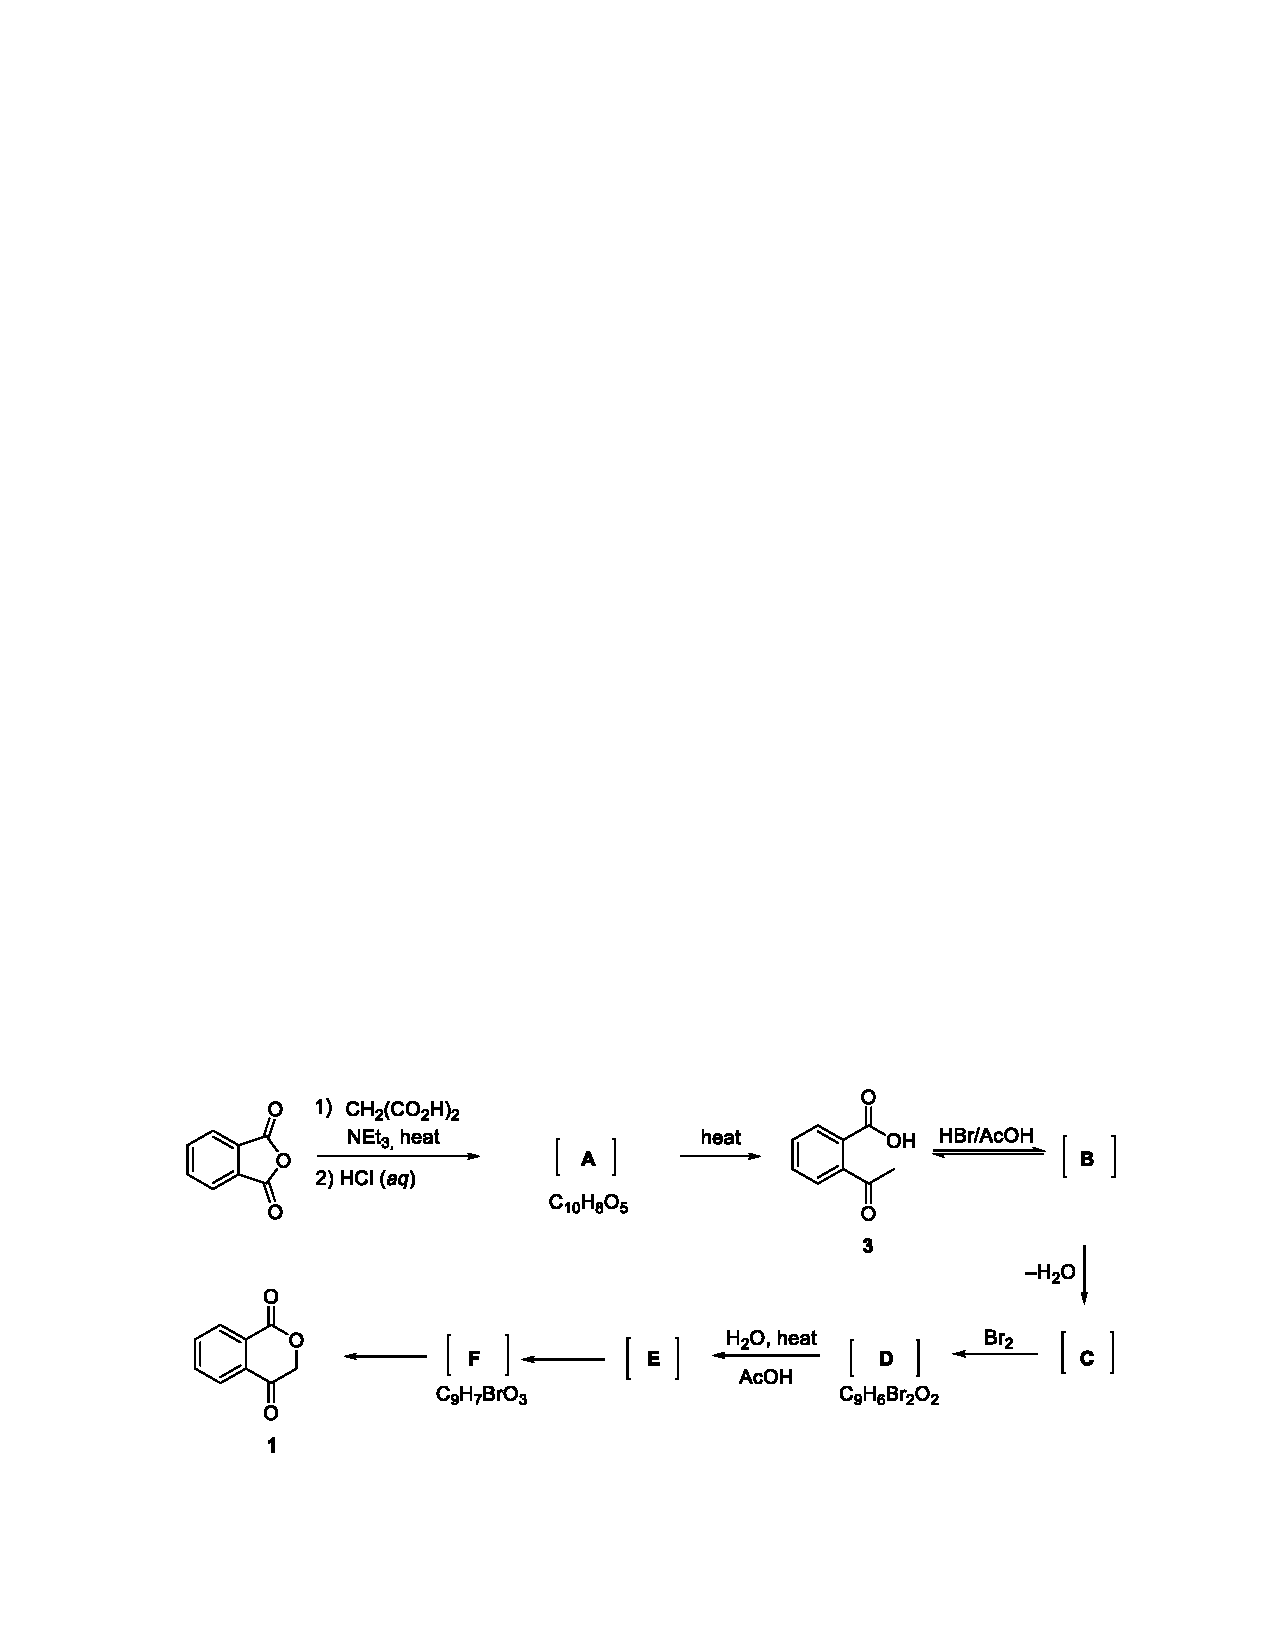
\includegraphics[width=16cm]{./pic/t6-2.pdf}
\end{figure}

中间体\textbf{B}和\textbf{C}的光谱数据:\textbf{B}:\textsuperscript{1}H NMR $\delta$ = 7.86-7.52 (4H), 4.13 (bs, 1H, 可与D\textsubscript{2}O交换), 1.97 (s, 3H). \textbf{C}:\textsuperscript{1}H NMR $δ$ = 7.92--7.58 (4H), 5.24 (m, 2H); \textsuperscript{13}C NMR δ = 166.8, 151.8, 139.0, 134.4, 130.4, 125.3, 125.1, 120.6, 91.3; MS m/z = 146.0

\noindent\textbf{6.1.} 画出在\textbf{1}的合成中中间体\textbf{A}-\textbf{F}的结构。

从环己烯开始可经由一系列关键步骤,包括傅-克酰基化反应、卤仿反应、还原反应和氧化反应合成关键化合物\textbf{2}。环己烯和乙酰氯进行傅-克酰基化反应生成氯代环己基甲基酮\textbf{J}。环己烯和乙酰氯的反应最初生成了碳正离子\textbf{G},随后连续进行了两次瓦格纳-梅尔外因重排先后生成分子式不变的碳正离子\textbf{H}和\textbf{I}。氯离子与碳正离子\textbf{I}反应生成了\textbf{J},\textbf{J}再与氯苯发生傅-克反应生成\textbf{K}。用次氯酸钠(NaOCl)与甲基酮\textbf{K}进行卤仿反应生成相应的酸\textbf{L},\textbf{L}再经由多步反应转化为醛\textbf{2}。

\noindent\textbf{6.2.} 画出分子式相同的碳正离子\textbf{G}-\textbf{I}的结构式。

\begin{figure}[h]
	\centering
	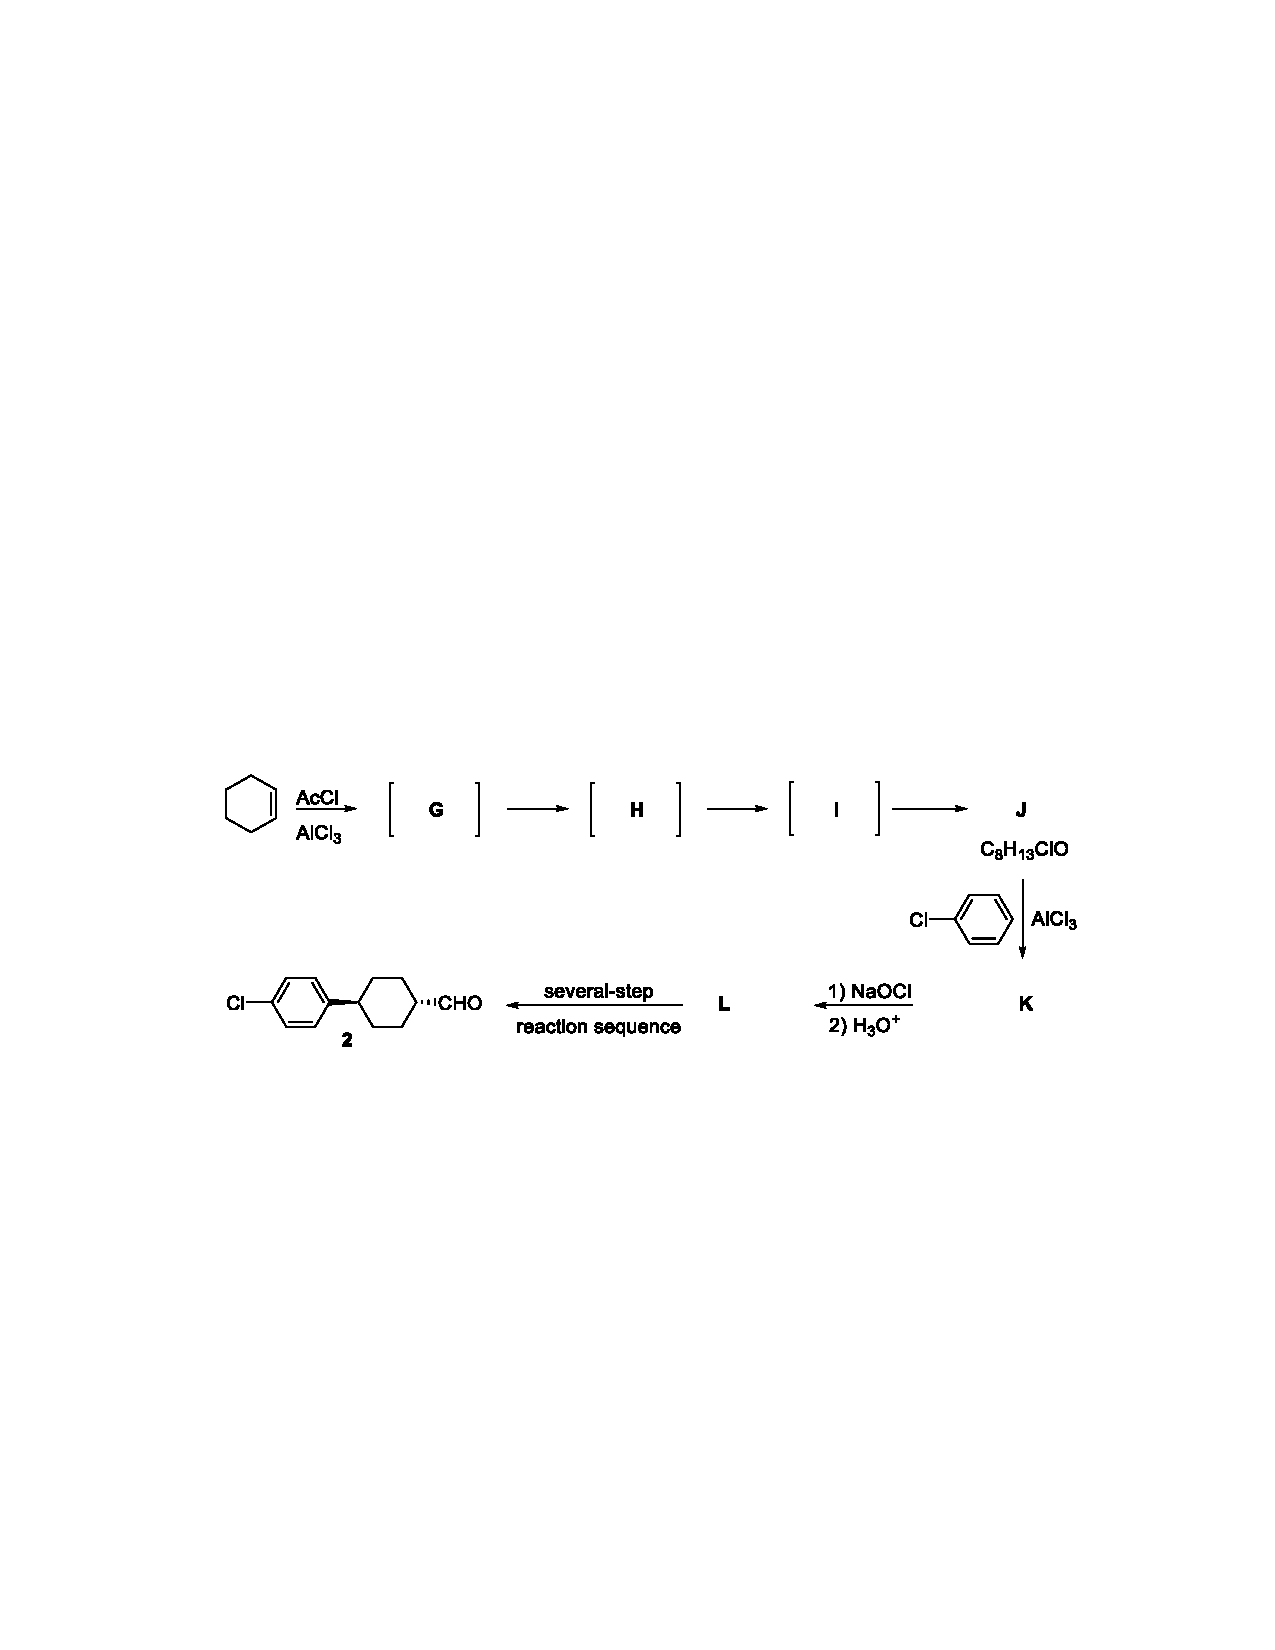
\includegraphics[width=15cm]{./pic/t6-3.pdf}
\end{figure}

\noindent\textbf{6.3.} 碳正离子\textbf{G}-\textbf{I}有手性吗?

\noindent\textbf{6.4.} 画出化合物\textbf{J}-\textbf{L}的结构。

\noindent\textbf{6.5.} 选出所有正确的选项。

\renewcommand{\labelitemi}{$\square$}
\begin{itemize}
	\item \textbf{L}有四个立体异构体。
	\item \textbf{L}是一个手性化合物。
	\item \textbf{L}是一个非手性化合物。
	\item \textbf{L}是一个内消旋化合物。
	\item \textbf{L}有两个立体异构体。
	\item \textbf{L}的立体异构体之间是非对映异构体。
	\item \textbf{L}的立体异构体之间是对映异构体。
\end{itemize}
\renewcommand{\labelitemi}{$\bullet$}

\noindent\textbf{6.6}下列化合物中哪个或哪些在卤仿反应中生成?

\renewcommand{\labelitemi}{$\square$}
\begin{itemize}
	\item CH\textsubscript{2}Cl\textsubscript{2}
	\item CH\textsubscript{3}Cl
	\item CHCl\textsubscript{3}
	\item CCl\textsubscript{4}
\end{itemize}
\renewcommand{\labelitemi}{$\bullet$}

\newpage\noindent\textbf{6.7}下列由化合物\textbf{L}生成醛\textbf{2}的反应条件有哪些是正确的?选出所有的正确答案。

\begin{figure}[h]
	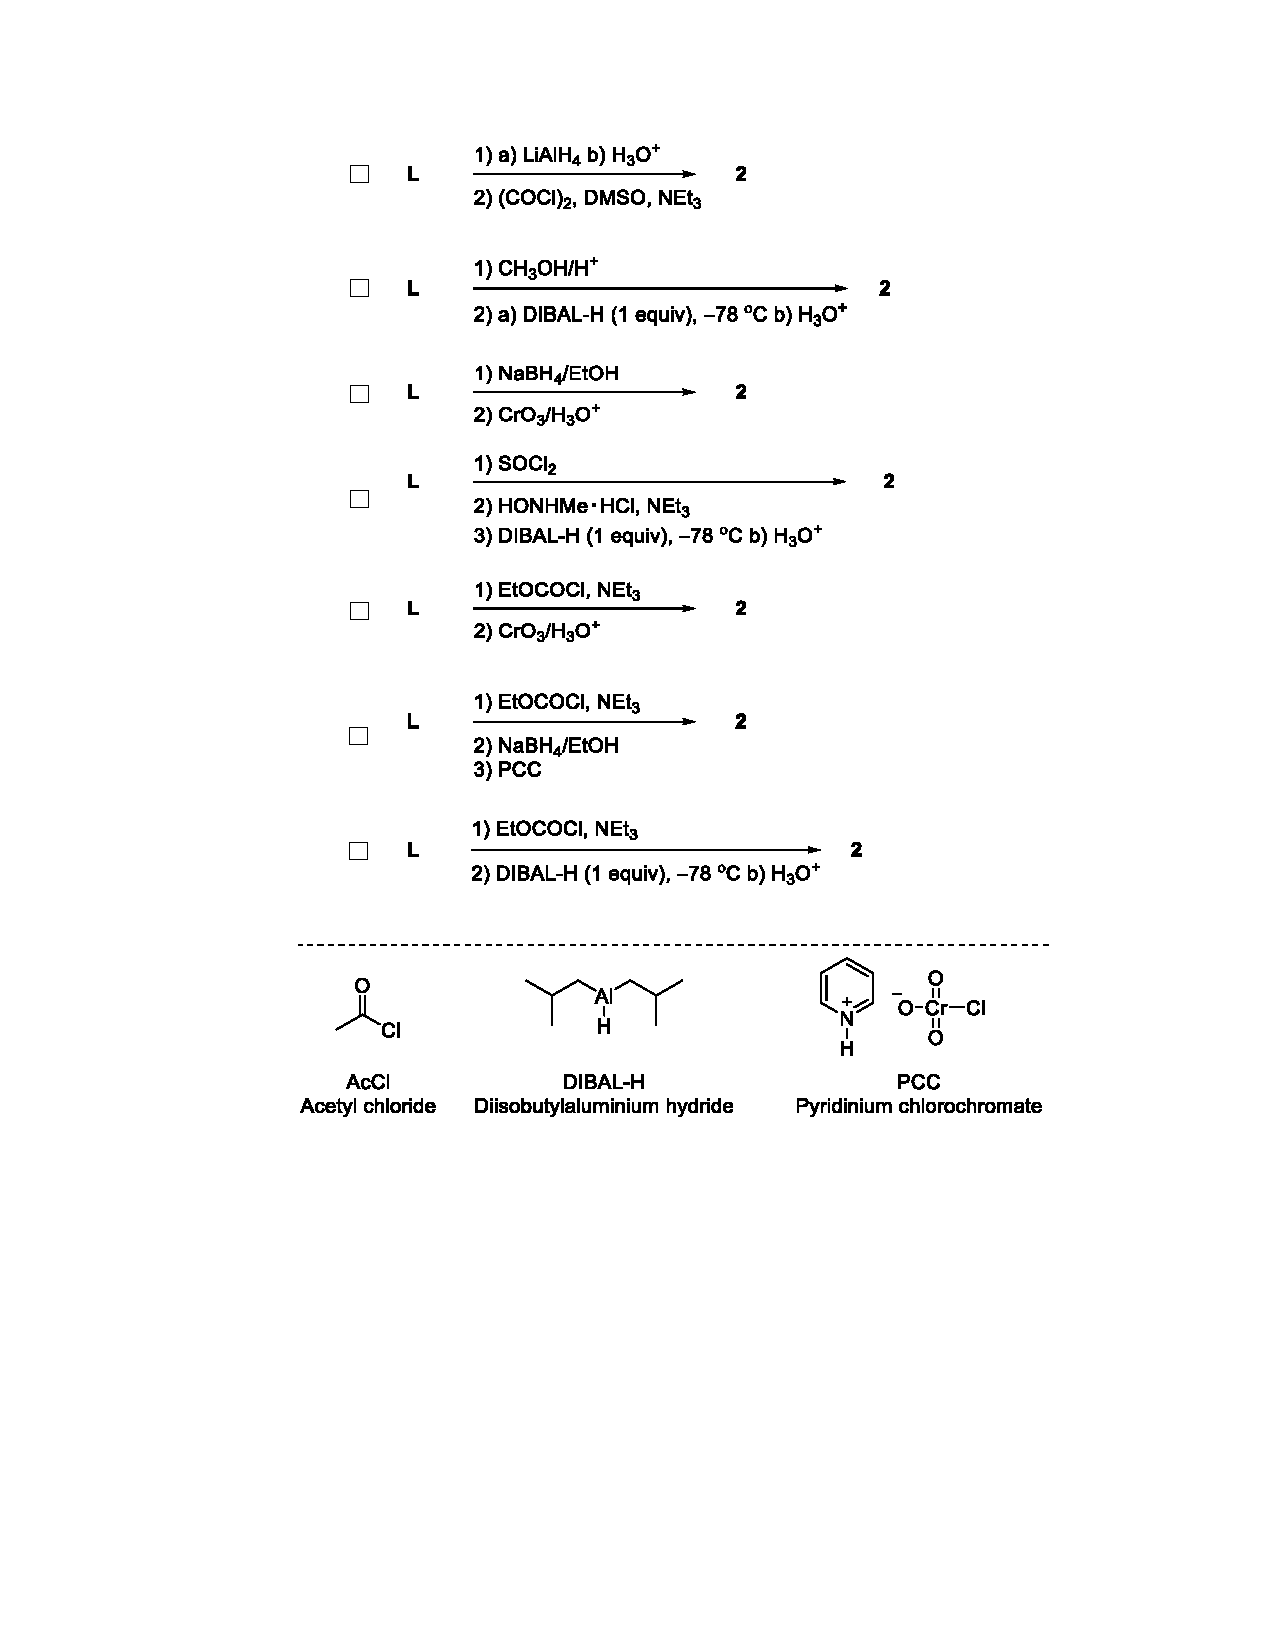
\includegraphics[width=14cm]{./pic/t6-4.pdf}
\end{figure}

